\documentclass[tikz]{standalone}
\usepackage[compat=1.1.0]{tikz-feynman}

\begin{document}

% gluon fusion
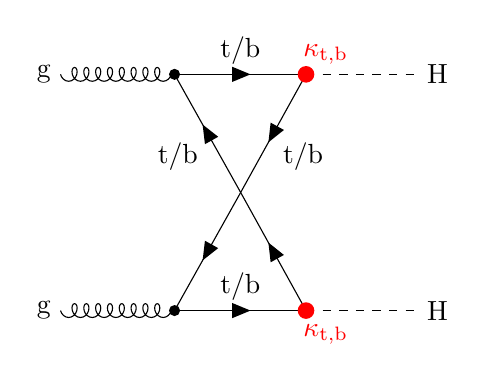
\begin{tikzpicture}
  \begin{feynman}
    \vertex at (0,3) (top) {g};
    \vertex at (0,0) (bot) {g};
    \vertex at (2.5,1.5) (mid);
    \vertex at (1.66,3) (box1);
    \vertex at (1.66,0) (box2);
    \vertex at (3.33,3)  (box3);
    \vertex at (3.33,0)  (box4);
    \vertex at (5, 3) (h1) {H};
    \vertex at (5, 0) (h2) {H};
    
    \diagram* [horizontal=mid to h] {
      (top) -- [gluon] (box1),
      (bot) -- [gluon] (box2),
      (box1) -- [fermion, edge label = t/b] (box3) -- [fermion, edge label = t/b] (mid) -- [fermion] (box2) -- [fermion, edge label = t/b] (box4) -- [fermion] (mid) -- [fermion, edge label = t/b] (box1),
      (box3) -- [scalar] (h1),
      (box4) -- [scalar] (h2),
    };
  \end{feynman}

  \fill[red] (box3) circle (3pt);
  \node[red] at ($(box3) + (0.25,0.25)$) {$\kappa_{\mathrm{t},\mathrm{b}}$};
  \fill[red] (box4) circle (3pt);
  \node[red] at ($(box4) + (0.25,-0.3)$) {$\kappa_{\mathrm{t},\mathrm{b}}$};
  \fill[black] (box1) circle (2pt);
  \fill[black] (box2) circle (2pt);
\end{tikzpicture}

\end{document}
